\documentclass{IEEEtran}

\usepackage{hyperref}
\usepackage{listings}
\usepackage{graphicx}
\graphicspath{{img/}}

\title{Florida Polytechnic University Campus-Wide Mesh Network}
\date{2015-07-17}
\author{Joseph Prine, John McCormack, Cody Madden, William Mathis, Ryan Integlia}

\begin{document}
\maketitle

\begin{abstract}
Abstract—The Florida Polytechnic University campus-wide mesh network will serve as an educational tool and research platform for students to develop network applications, technologies, and experiments.  As an educational tool, the network will provide students with hands-on experience in the development of sensor networks, as well as the exploration of software-defined radio and software-defined networks.  As a research platform, students will be able to develop applications and technologies related to gaming, social media, and security.
\end{abstract}
\begin{IEEEkeywords}
Index Terms—Software Defined Radio, ad-hoc network, mesh network
\end{IEEEkeywords}

\section{Introduction}
	
	Wireless networks are quickly becoming a necessary infrastructure for the 21st century.  A reliable connection to the internet, or to specific intranets, is as critical as a connection to an electrical power grid for a growing number of applications.  Aside from the obvious network applications like communication and security, new ways to use networks are becoming more popular.  These applications include social networking, gaming, smart manufacturing, and smart devices like intelligent cars and wearable technology. Reliable, robust, and abundant wireless networks will allow a wide array of devices to communicate with each other, making the Internet of Things possible.

\section{Network Architecture}

	The Florida Polytechnic University Mesh Testbed essentially takes the form of a mobile ad-hoc network, or MANET.  The wireless multi-hop communication of the mesh network, communicating with the world wide web via multiple gateway nodes, forms a flexible network for communication. The network is currently made up of several small, battery operated wireless routers running OpenWRT. OpenWRT is an open source, freely available operating system with a large community of developers. Batman-adv is used as the mesh routing protocol. This can be seen in Figure 1.  

\begin{figure*}
	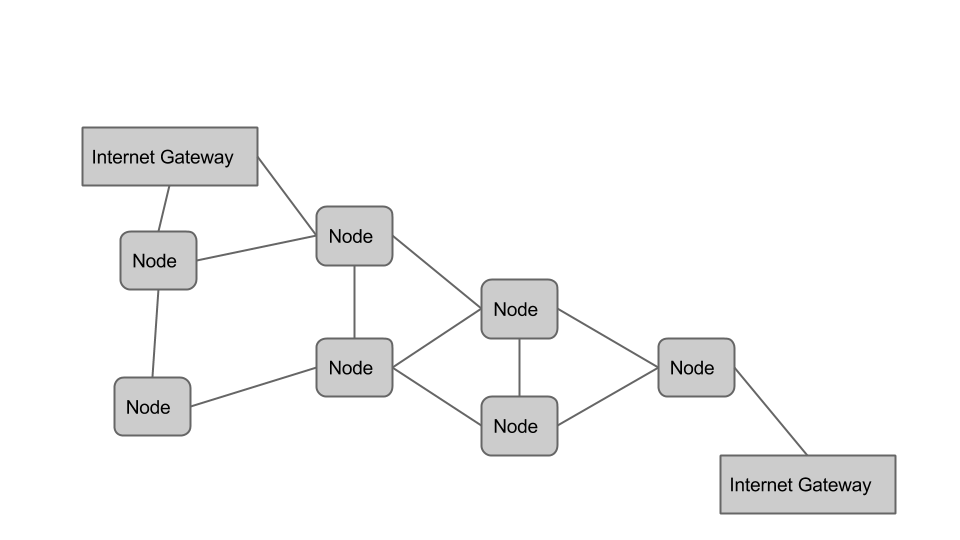
\includegraphics[width=\textwidth]{nodearchitecture}
	\caption{A brief overview of the mesh architecture}
\end{figure*}
\section{Data Collection}

The goal of the mesh network is to implement a distributed, wireless, data collection platform. Currently, Raspberry Pi microcomputers are connected to various sensors. The Raspberry Pi’s can then utilize the mesh network to send the data to a central server for storage and processing. The Raspberry Pi is an open source, low power, microcomputer that allows us to collect more data than would be possible on a simple microcontroller. However, because batman-adv present the network transparently to the computer, it would be possible to switch to a microcontroller without any change to the rest of the infrastructure. This would allow for data collection over a longer period of time, with less resources. 

\section{Future Work}
\subsection{Data Visualition}
	
	Pure data is rarely helpful on its own. Being able to interpret the data is what is useful and interesting. We are working towards creating a visualization system within the Unity game engine. Unity is not open source, but it is freely available and feature the ability to compile for nearly every major computer, mobile, and video game platform. We currently have a demonstration that allows for a button to be pressed on a raspberry pi, which then triggers a virtual LED in Unity to change colors. A button can then be pressed within Unity to change the color of an LED on the raspberry pi. This was tested and found to work over the mesh network. As the available tools for data collection increases, we will be able to increase the available options for data visualization. 

\subsection{Data Interaction}

In order to make the interaction with the data more natural and innovative, we will seek to employ various hardware interaction devices with the Unity system. We have begun to experiment with the Myo Armband, Neurosky EEG device, Leap Motion Plus, and 2D Lidar systems. Each of these tools presents a unique human computer interaction (HCI) method that could allow a user to go beyond a normal mouse and keyboard setup. These systems could also be paired with an Oculus Rift virtual reality headset to give the user the ability to entirely immerse themselves in the data visualization environment.  

\subsection{Software Defined Radio and Cognitive Networks}

	To increase the security, network reliability, and scalability of the platform, we will look to use software defined radios to create a cognitive mesh network. Software defined radios abstract most of the components of a wireless transceiver into software. This allows them to act as many different types of radios over a wide range of frequencies. By scanning the adjacent area for open frequencies, the mesh network could be designed to hop from frequency to frequency. This allows the radios to always communicate in a free band without interrupting any other transmissions. We are currently exploring the use of GNU Radio for cognitive networks and have successfully run some basic SDR tests using this free and open source software tool. 

\subsection{Robotic Control over the Mesh Network}

	One of the most exciting applications of the mesh network is for the distributed control of robots including Unmanned Aerial Vehicles (UAVs) and Unmanned Submersible Vehicles (USVs). Research has begun at other universities into controlling UAVs using this type of network, however almost all of it is in the simulation level. Florida Polytechnic could become the leader in this quickly emerging field. A base station could be established within the VTC or a similar lab space on campus. Once connected to the node, commands could be sent to the robot, while live data is returned to the base station for processing. Color changing smart lighting on the node could change to indicate which node is currently connected to the UAV. While not strictly necessary, this would allow students to see a visualization of packets flowing through the mesh. 

This concept could be expanded to swarm robotics. A huge portion of the research involved in swarm robotics is on intraswarm communication. In order for the group to function, appropriate information must be able to flow through the swarm. The mesh nodes would allow this data to be transported over a wide area from robot to robot. Human Swarm Interaction is also an emerging field. The VTC could be given proper equipment to allow work to be done in this field. A system involving an oculus rift and a joystick or gamepad could be used to create a simulated cockpit. Users could then watch the gross movement of the swarm on projectors in the VTC. These projectors could show where on a map the robots are as well as stream live video feed from the group. Pilots could then use the rift and joystick to control specific robots.


\end{document}
